\documentclass[../thesis.tex]{subfiles}
\begin{document}
\chapter{Organic Light-Emtting Devices}\label{sec:oleds}

\section{Architecture and Basic Operation} \label{sec:oled_operation}

\begin{wrapfigure}{r}{.5\textwidth}
\centering
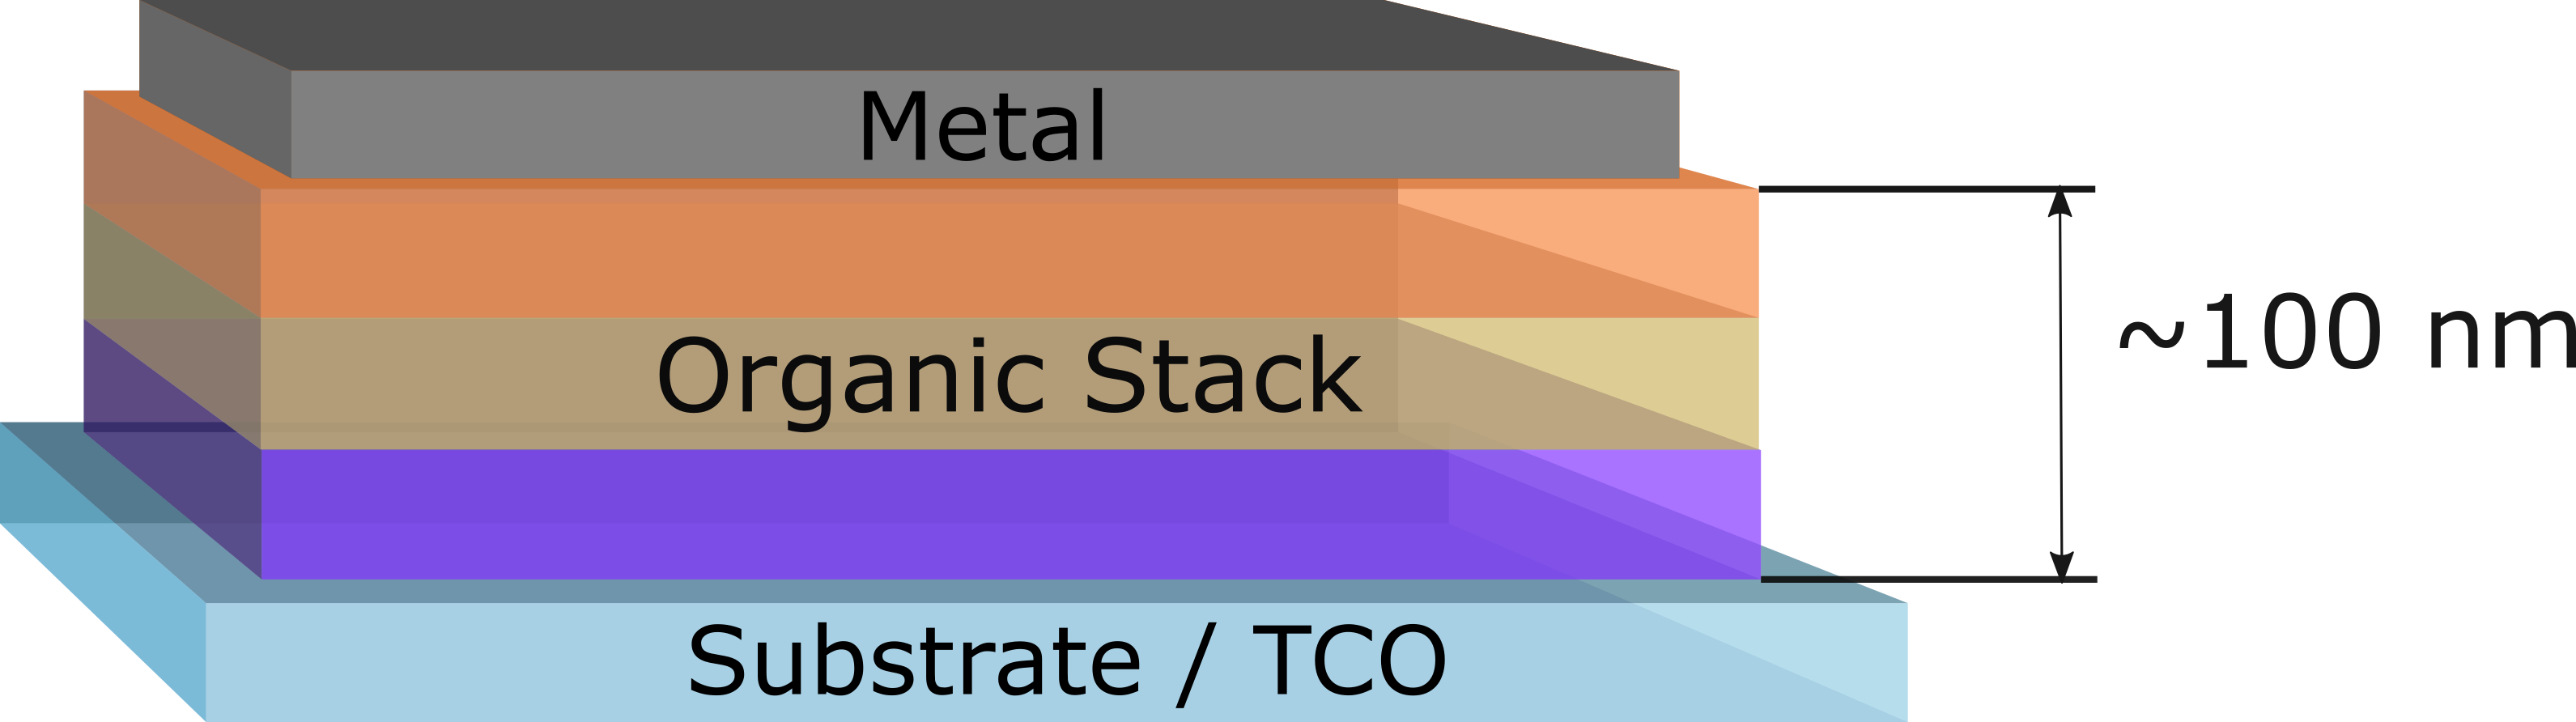
\includegraphics[width=.48\textwidth]{oleds/layer_diagram}
\caption{Basic layer diagram for OLED devices.}
\label{fig:oleds_layer_diagram}
\end{wrapfigure}

Organic Light Emitting Devices (OLEDSs) consist of an organic layer stack sandwiched between two electrodes.
For light to escape, one of the electrodes is transparent, and in most lab scale devices, this is the bottom contact.
This is often accomplished by using glass coated with Indium Tin Oxide (ITO) as a transparent conducting material.
The opposing contact is typically a metal, and in most cases Aluminum.
An example of this type of structure is shown in Figure \ref{fig:oleds_layer_diagram}.

The organic stack of devices is typically 80 nm or more and consists of multiple layers.
Detailed device operation will be expanded upon in Chapter \ref{sec:unified}, but the goal of the layer stack is to efficiently form and recombine excitons.
When voltage is applied, electrons are injected from the metal contact into the electron transport layer (ETL) and holes are injected from the ITO into the hole tranport layer (HTL).
Carriers transport through these layers to a region where exciton formation is designed to occur.  
This can be done in a variety of ways and is discussed in detail in Section \ref{sec:oled_history}, but most modern devices use a structure with a dedicated emissive layer (EML), as shown in Figure \ref{fig:oleds_energy_level_diagram}.
In this type of device, the emitter molecule or guest, is doped at low concentration within a host matrix.\supercite{Baldo2000}
This composite film structure is used because most emissve molecules show a reduction in \pl with increasing concentration.\supercite{Turro1991a}
The host molecule is used to help transport charge to the emissive molecule and separate the guest molecules.
The host molecule is designed to have a wider energy gap, making it energetically favorable for excitons to form on the guest molecule.

\begin{figure}[ht]
\centering
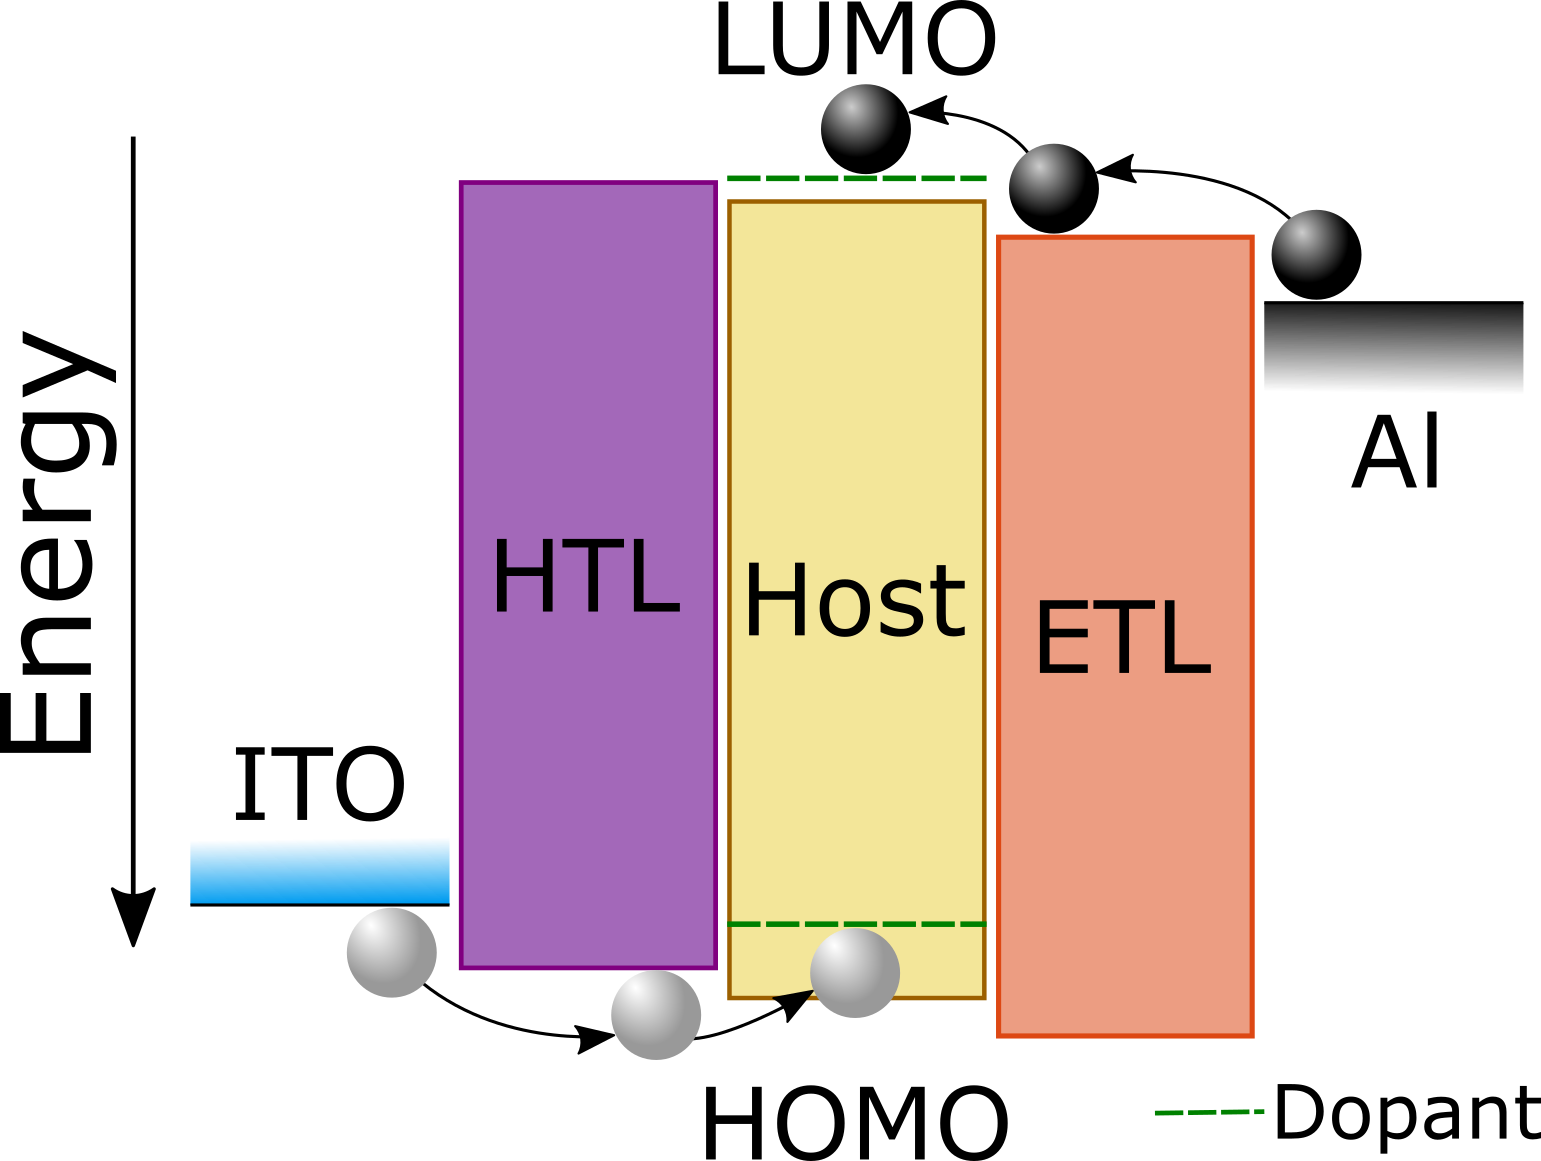
\includegraphics[width=.8\textwidth]{oleds/energy_diagram}
\caption{Energy level diagram of an OLED.  Energy is shown in reference to the vacuum level.  Electrons are shown in black spheres, holes shown in white.}
\label{fig:oleds_energy_level_diagram}
\end{figure}

The structure shown in Figure \ref{fig:oleds_energy_level_diagram} is greatly simplified from most devices.
Injection layers (HIL/EIL) are often used to aid in charge injection into the device between the electrode and transport materials.
These materials will sit energetically between the electrode and the transport layer.
To confine charges within the EML, blocking layers (HBL/EBL) are often used between the EML and the opposing transport layer.
For example, a hole blocking layer would sit between the EML and the ETL and would have an energy level simlar to the ETL, so electron transport would not be disrupted, but would have a high HOMO energy or a low hole mobility.
These types of layers are often added as needed based on the energetic levels of the other materials in use.

\subsection{Efficiency}

\begin{figure}[ht]
\centering
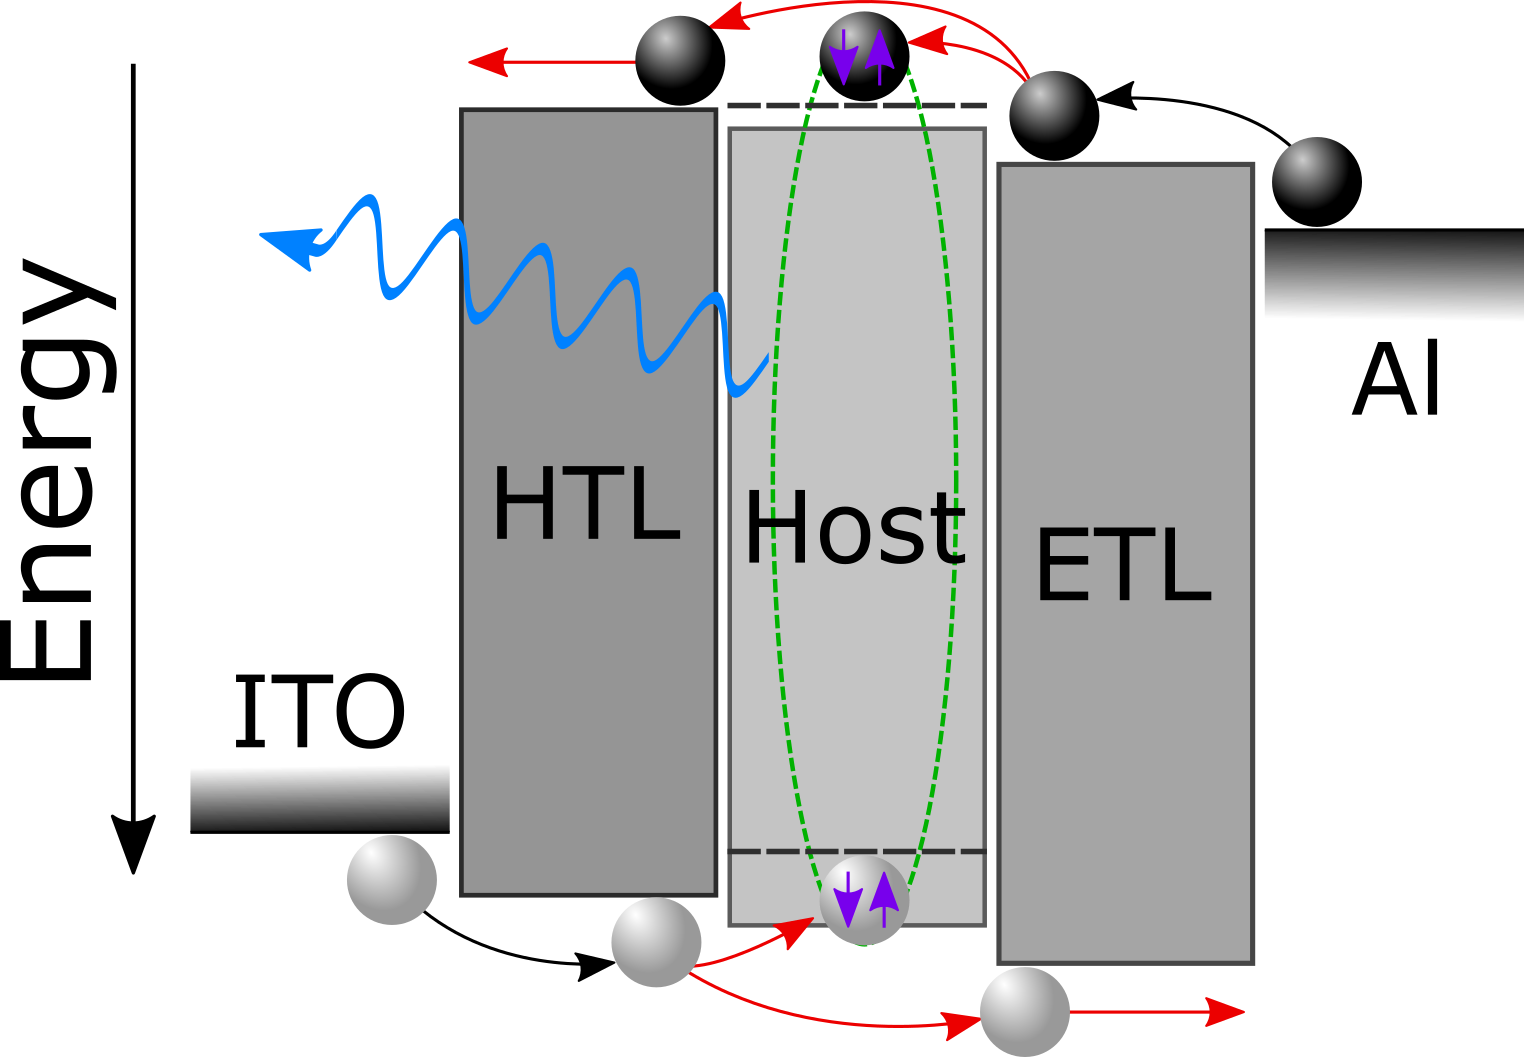
\includegraphics[width=.8\textwidth]{oleds/energy_diagram_EQE}
\caption{External Quantum Efficiency on energy level diagram.  \oc represented in blue, \pl in green, $\chi$ in purple, and \ef in red.}
\label{fig:oleds_energy_level_diagram_EQE}
\end{figure}

Device efficiency is often thought of as a four component process as:\supercite{Baldo1998a}

\begin{equation}
\eqe=\chi\pl\ef\oc
\label{eqn:eqe}
\end{equation}

The efficiency with which injected charges form excitons is the exciton formation efficiency, \ef (traditionally called charge balance,$\gamma$).
This is competitive with charge loss through the device and is shown in red in Figure \ref{fig:oleds_energy_level_diagram_EQE}.
In modern devces, \ef can approach 100\% at the maximum effciency point.
Electrically, excitons are formed in a 3:1 Triplet:Singlet ratio, as discussed in Chapter \ref{sec:excitons}.
The radiative spin fraction, $\chi$, captures the fraction of these formed excitons that are able to emit.
For fluorescent materials, $\chi=1/4$ and for phosphorescent materials, $\chi=1$.
The photoluminescence efficiency, \pl is the efficiency of photon generation from the radiatively allowed excitons and can reach 100\%
The out-coupling efficiency, \oc, is the fraction of photons that escape the device in the forward viewing direction, and is competitive with wave-guided modes and surface plasmons.\supercite{Furno2010,Furno2012}
For most devices \oc is the limiting process for efficiency, and typically is limited to 20-30\%, but can be aided by enhancing films or layers.


\section{Fabrication Processes}

Substrates consist of glass precoated with indium-tin oxite (ITO).  
Prior to deposition, substrates are cleaned using 5 minutes each of sonicated Tergitol, water, and two cycles of acetone, followed by two cycles of boiling isopropynal.  
This is followed by a UV-ozone treatment for 10 minues.  
Large area devices on patterned ITO are spin coated with a solution processed hole conducting planarizing layer.
In my time in the group, this started with Pedot-PSS and has transitioned to the more commercially used Plexcore AQ-1200.
Pedot-PSS is water based and seemed more susceptible to treatment conditions prior to deposition, such as freezing.
AQ-1200 has been a more reliable material.
AQ-1200 has been replaced with AQ-1250, which appears to be the same formula, but with tighter control over consistency.
For all solution processed layers, spin coating is done for 30 seconds at 3000 rpm, followed by a 30 minute bake at 150 $^\circ$C.

\begin{figure}[ht]
    \centering
    \begin{subfigure}{.3\textwidth}
    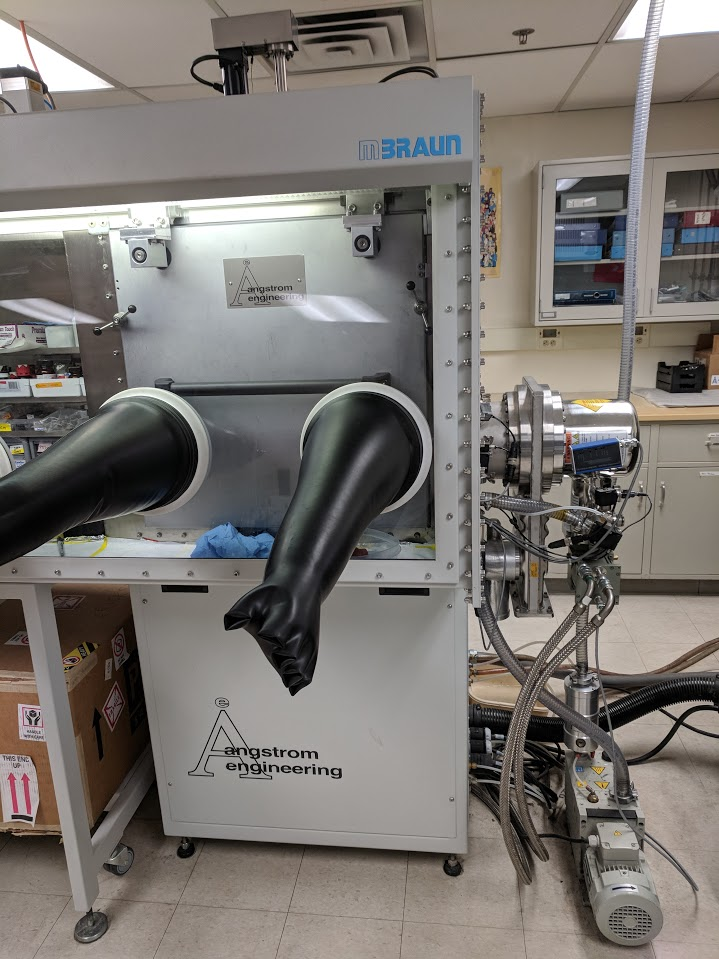
\includegraphics[width=\textwidth]{oleds/chamber}
    \caption{}
    \label{fig:oleds_angstrom}\par\vfill
    \end{subfigure}
    \begin{subfigure}{.3\textwidth}
    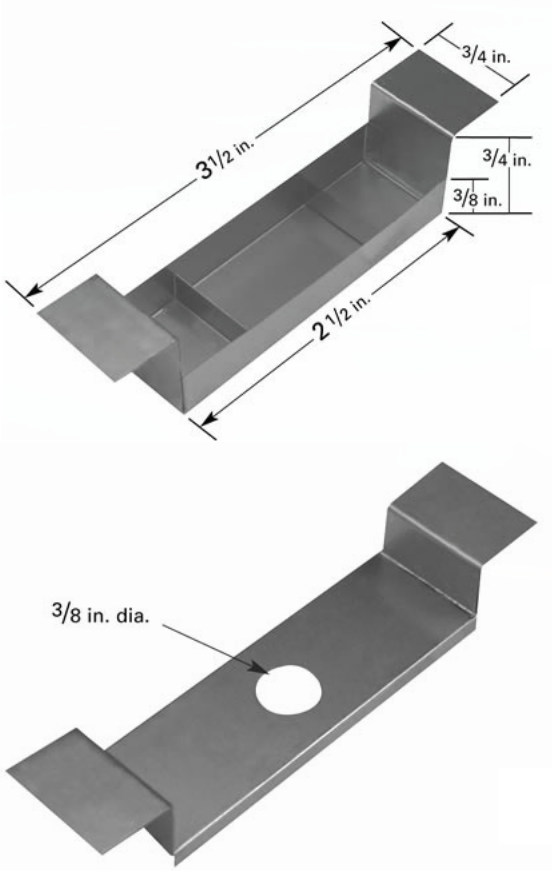
\includegraphics[width=\textwidth]{oleds/dep_boat}
    \caption{}
    \label{fig:oleds_deposition_boat}
    \end{subfigure}
    \begin{subfigure}{.3\textwidth}
    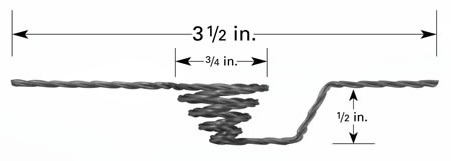
\includegraphics[width=\textwidth]{oleds/al_boat}
    \caption{}
    \label{fig:oleds_al_boat}
    \end{subfigure}
\caption{a. Angstrom vacuum chamber b. Organic deposition boat c. Aluminum deposition boat}
\end{figure}

Within our lab, the standard fabrication process for OLEDs is thermal evaporation at base pressures <10$^{-7}$ Torr.  
This is done in an Angstrom Engineering vacuum deposition chamber from tungston boat sources for organic materials, shown in Figures \ref{fig:oleds_angstrom} and \ref{fig:oleds_deposition_boat}, respectively.
Material deposition rates can be measured using quartz crystal monitors (QCMs) during deposition.
The absolute rate of material deposition can be calibrated by conducting ellipsometry on grown films to determine thickness.
This chamber allows simultaneous deposition of up to 4 materials at a time.
Codeposition of materials allows for the creation of doped layers, which can even be varied with time to create graded composition profiles.
For most devices, cathodes consist of 1 nm of lithium fluoride, from a dimple boat, followed by 100 nm of Aluminum, from the boat shown in Figure \ref{fig:oleds_al_boat}.

For unpatterned devices, the whole substrate is coated in ITO, and device pixels are formed using a metal mask that defines the device area.
In this case, to contact devices, contact must be made with the ITO for the anode and the Al cathode.
A hard metal probe is used to contact the ITO by poking through the organic stack.
However, the metal must be contacted without damaging the metal or underlying organic stack, as any damage would disrupt the device behavior, and at worst, short the contact to the ITO anode.
In order to contact the metal, a 100$\mu$ gold wire is used to gently contact the metal surface.

\begin{figure}[ht]
    \centering
    \includegraphics[width=.7\textwidth]{oleds/masks}
    \caption{a. ITO Pattern b. Organic Mask c. Metal Mask d. Mask Overlays.  Device area shown in red.}
    \label{fig:oleds_masking}\par\vfill
\end{figure}

Patterned devices consist of a patterned ITO substrate with a corresponding patterned metal mask, where the intersection forms the device area.
To ease contacting, an ITO pad is typically placed below the metal at the contact point outside of the organic deposition region as demonstrated in Figure \ref{fig:oleds_masking}.
This method allows for contacting the device off of the device active area, and does not suffer from the difficulty of contacting and is essential for devices to be encapsulated.
In this case, it is important to consider lateral transport within the HIL.
A sharp edge on the ITO pattern can result in a discontinuity of the organic stack at the device edges and can frequently short the device with metal directly in contact with the ITO.
To prevent this, a planarizing layer is used which minimizes the effects of ITO roughness and the discontinuity of the step edge.
While this is effective, planarizing layers are designed to have high mobility and lateral conduction could become important as it may lead to shorting between the anode and cathode ITO pads.
To prevent this in our devices, the planarizing layer is disturbed between the two pads in order to disrupt lateral transport.

For device lifetimes, to minimize oxygen exposure, devices are packaged.
This is done before devices are exposed to oxygen levels outside of a glovebox.
A UV cured epoxy seal is formed around the device active area and is capped with a glass microscope slide cover slip.
The epoxy is then cured with 3 minutes of exposure to a UV lamp.
For extreme long lived devices or higher shelf life, a dessicant can be used, but this is not common in our lab due to the relatively short lifetimes that we are studying.


\section{Characterization}

Though numerous characterizations exist to analyze devices, the standard metrics of performance consist of current-voltage, luminance, and efficiency.
Luminance is typically calculated in candellas per meter squared ($cd/m^2$).
There are three common efficiency metrics for devices, including the external quantum efficiency (\%), the power efficiency ($W/W$) and the luminance efficiency (lm/W).
Though dependent on field of study, for academic OLED interests, the most commonly explored metric is the external quantum efficiency (\eqe).

\subsection{Current Voltage and Luminance}

\begin{wrapfigure}{r}{.5\textwidth}
    \centering
    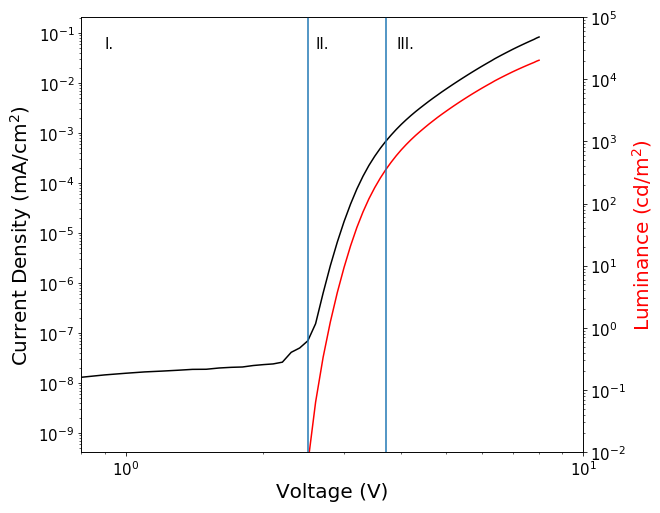
\includegraphics[width=.48\textwidth]{oleds/ivl}
    \caption{a. Device current voltage  and luminance voltage behavior}
    \label{fig:oleds_ivl}\par\vfill
\end{wrapfigure}

The current-voltage behavior of most OLEDs follows a diode-like current-voltage dependence.
This is characterized by a weak dependence of current on voltage below some threshold, followed by a strong dependence at high voltage, as shown in Figure \ref{fig:oleds_ivl}.
In terms of device operation, at low voltage below turn-on (Region I), carriers do not have enough energy to make the transitions between molecular orbital energy levels and cannot be injected into the device.
Soon after turn on, carriers are overcoming the injection barriers of the material stack and in an ideal device, forming a strong recombination current for light emission (Region II).
In this region, the current is limited by carrier injection and follows an exponential dependence as carriers overcome the injection barrier potential.\supercite{Pope1999}
At high voltage, injection barriers have been overcome and there is a charge buildup in the device which limits the current.
This region is known as the space-charge limit and the current-voltage characteristic shows a power law dependence.\supercite{Pope1999,Mark1962,Lampert2002a}
In a well formed device, luminance should closely follow current, as most current should be going to recombination and exciton formation.

For device brightness characterization, either optical power or luminance can be used.
Optical power is simply a characterization of the total photon power exiting a device.
This is typically calculated by measuring the total device light output using a large area photodiode.
For optical power or optical power density measurements, it is important to know the measured light producing region being measured.
This can either be done by ensuring the total device area and all light output is measured, in which case the area of interest is the device area, or by measuring a known subsection of the device.
The current output by the detector can be related to the incident optical power by the responsivity function of the detector, reported as a function of wavelength as $W/A$.
A typical responsivity for a silicon detector is shown in Figure \ref{fig:oleds_responsivity}a.

\begin{wrapfigure}{r}{.5\textwidth}
    \centering
    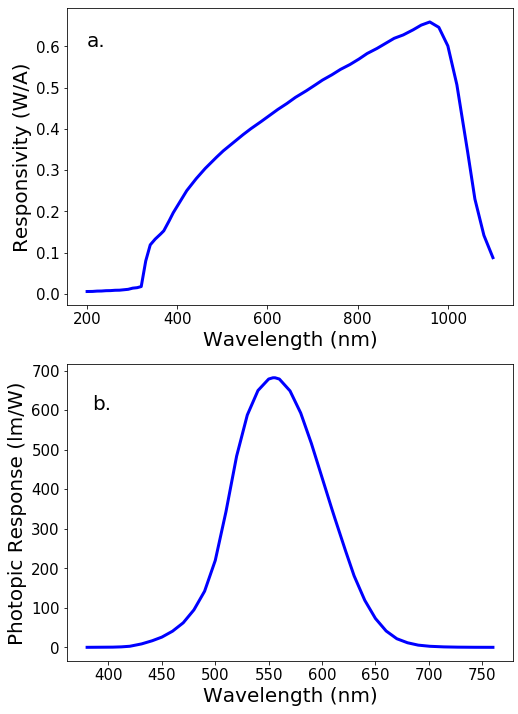
\includegraphics[width=.48\textwidth]{oleds/responsivity}
\caption{a. Silicon detector responsivity b. Photopic response}
\label{fig:oleds_responsivity}
\end{wrapfigure}


Luminance is reported in candelas per meter squared ($cd/m^2$), sometimes called a 'nit'.
The candela is a measure of perceived light intensity per solid angle and is equivalent to 1 candle power.
To measure luminance, the light output must be normalized to the wavelength dependent response of the human eye, known as the photopic response, shown in Figure \ref{fig:oleds_responsivity}b.
This is typically done in one of two ways.
The first method (employed by our group) is to use a spectrometer to measure the output light spectrumin Watts per nanometer.  
Then the spectrally averaged photopic response can be found for the light source of interest.
Then, the output optical power can be measured by a simple photodiode and calibrated using the average photopic response.
Alternatively, a photodiode can be filtered and modified so that the responsivity function matches the photopic response.
In this case, the photodiode would directly output the luminance.
Both methods are standardly used in research groups.\supercite{Hershey2016,Inoue2016,Forrest2003}


\subsection{Efficiency Analysis}\label{sec:efficiency_analysis}

As mentioned previously, there are three common measures of device efficiency.  
The first is power efficiency, measured in $W/W$.
This is straight forward to calculate given the previous discussion of measuring optical power.
The luminance efficiency $lm/w$ is related to the luminace output.
The lumen is a measure of total light output and is related to the candela by 1 lm = $2\pi$ candelas.
A keen eye would note that the candela is normalized per solid angle and a factor of $4\pi$ may be expected, but OLEDs are only able to emit in the forward direction.

The external quantum efficiecy (\eqe) is a measure of photons exiting the device per electron injected.
The photon flux out of the device can be calculated from the optical power by dividing by the average photon power, $hf_{avg}$, where $f_{avg}$ can be calculated from the measured spectrum.
The injected electron flux is simply $I/q$ where $I$ is the device current.
%The mathematical details of this model are discussed in detail by Forrest \textit{et al.}.\supercite{Forrest2003}
The mathematical details of this model are discussed in detail by \textcite{Forrest2003}.%\supercite{Forrest2003}


\section{Historical Developement}\label{sec:oled_history}
\subsection{The First OLEDs}

\begin{wrapfigure}{r}{.5\textwidth}
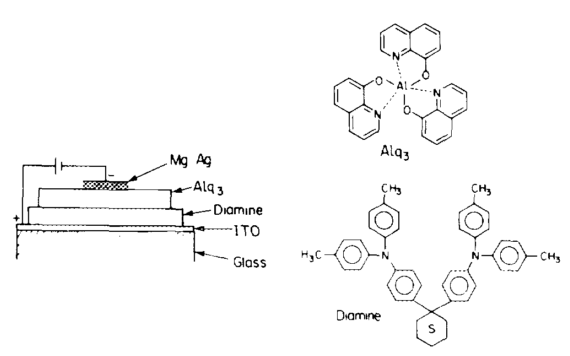
\includegraphics[width=.48\textwidth]{oleds/tang}
\caption{Structure of the first oled cell from \textcite{Tang1987}.  Diamine is commonly referred to now as TAPC.}
\label{fig:oleds_tang}
\end{wrapfigure}

Early interest in organic materials was generated based on use for organic laser dyes and the high fluorescence efficiency demonstrated.\supercite{Venkataraman1971,Schafer1977,Dresner1969}
Early attempts at producing electroluminescent devices tried contacting organic crystals, but required extremely high voltages to produce any light.\supercite{Williams1970,Helfrich1965}
The first successful OLED was demonstrated by \textcite{Tang1987} in 1987, one of the first to utilize vacuum deposition for thin films.
This was a bilayer device, with the structure shown in Figure \ref{fig:oleds_tang}, using TAPC at 75 nm thick and Alq$_3$ 60 nm, responsible for the emission of the device, centered around 550 nm.
These devices achieved \eqe $\approx$1\% and showed rapid degradaton.

In fluorescent cells, $\chi=0.25$ and without out-coupling enhancement $\oc \approx 0.20$, leaving a maximum \eqe of just 5\%.
Doped films were investigated soon after these initial findings in order to capitalize on the improved \pl at low concentration.\supercite{Tang1989a}
This host with emissive guest system is utilized by almost all devices.


\subsection{Phosphorescence}
\begin{wrapfigure}{r}{.5\textwidth}
%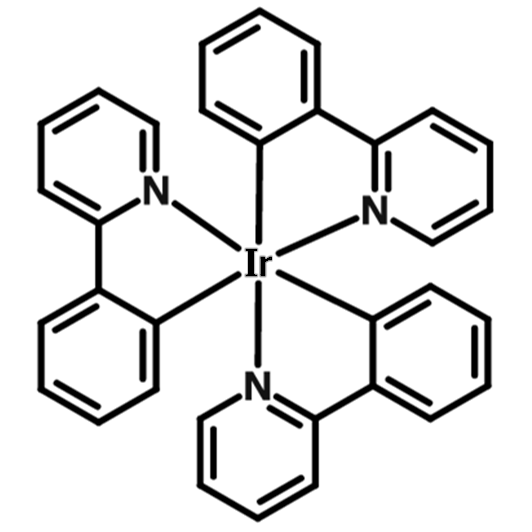
\includegraphics[width=.38\textwidth]{oleds/irppy3}
%\chemfig{Ir?-[::25,2]*6(-(-*6(=N?-=-=-))=-=-=)}
\chemfig{Ir?(-[:60,2]*6(-(-*6(=N?-=-=-))=-=-=))(-[:180,2]*6(-(-*6(=N?-=-=-))=-=-=))(-[:300,2]*6(-(-*6(=N?-=-=-))=-=-=))}
\caption{Molecular structure of the green phosphor, Ir(ppy)$_3$}
\label{fig:oleds_irppy}
\end{wrapfigure}
OLEDs saw a massive improvement in possible efficiency in 1998 with the introduction of phosphorescent dyes.\supercite{Baldo1998a}
These dyes use a heavy metal atom to create a metal-ligand charge transfer state, which allows mixing of the singlet and triplet states, and thus emission from the triplet exciton.
With all excitons able to emit, including the triplet state, the internal quantum efficiency ($\eta_{IQE}$) raises to 100\%.
These devices utilized the red phosphor PtOEP in conjunction with the laser dye DCM2.
This work comments on quenching at high current of the phosphor, a continuing problem which will be discussed further in Section \ref{sec:oleds_roll_off}.\supercite{Reineke2007,Hershey2016}
Pure red and green emission devices utilizing only a phosphorscent dopant were developed soon after, along with the development of the ubiquitous green emitter, Tris[2-phenylpyridinato-C$^2$,N]iridium(III) (Ir(ppy)$_3$), shown in Figure \ref{fig:oleds_irppy}.\supercite{OBrien1999a,Adachi2000}


Since the realization of the phosphorescent OLED, internal quantum efficiencies nearing 100\% for green, red, blue, and white devices have been demonstrated.\supercite{Su2008a,Erickson2010}
With high efficiency achieved, attention has shifted to maximizing lifetimes.\supercite{Scholz2008}
Despite the high efficiency of blue phosphorescent devices, lifetimes still remain limiting and blue fluorescent materials are still used in commercial technologies.


\subsection{Thermally Activated Delayed Fluorescence}

\begin{wrapfigure}{r}{.5\textwidth}
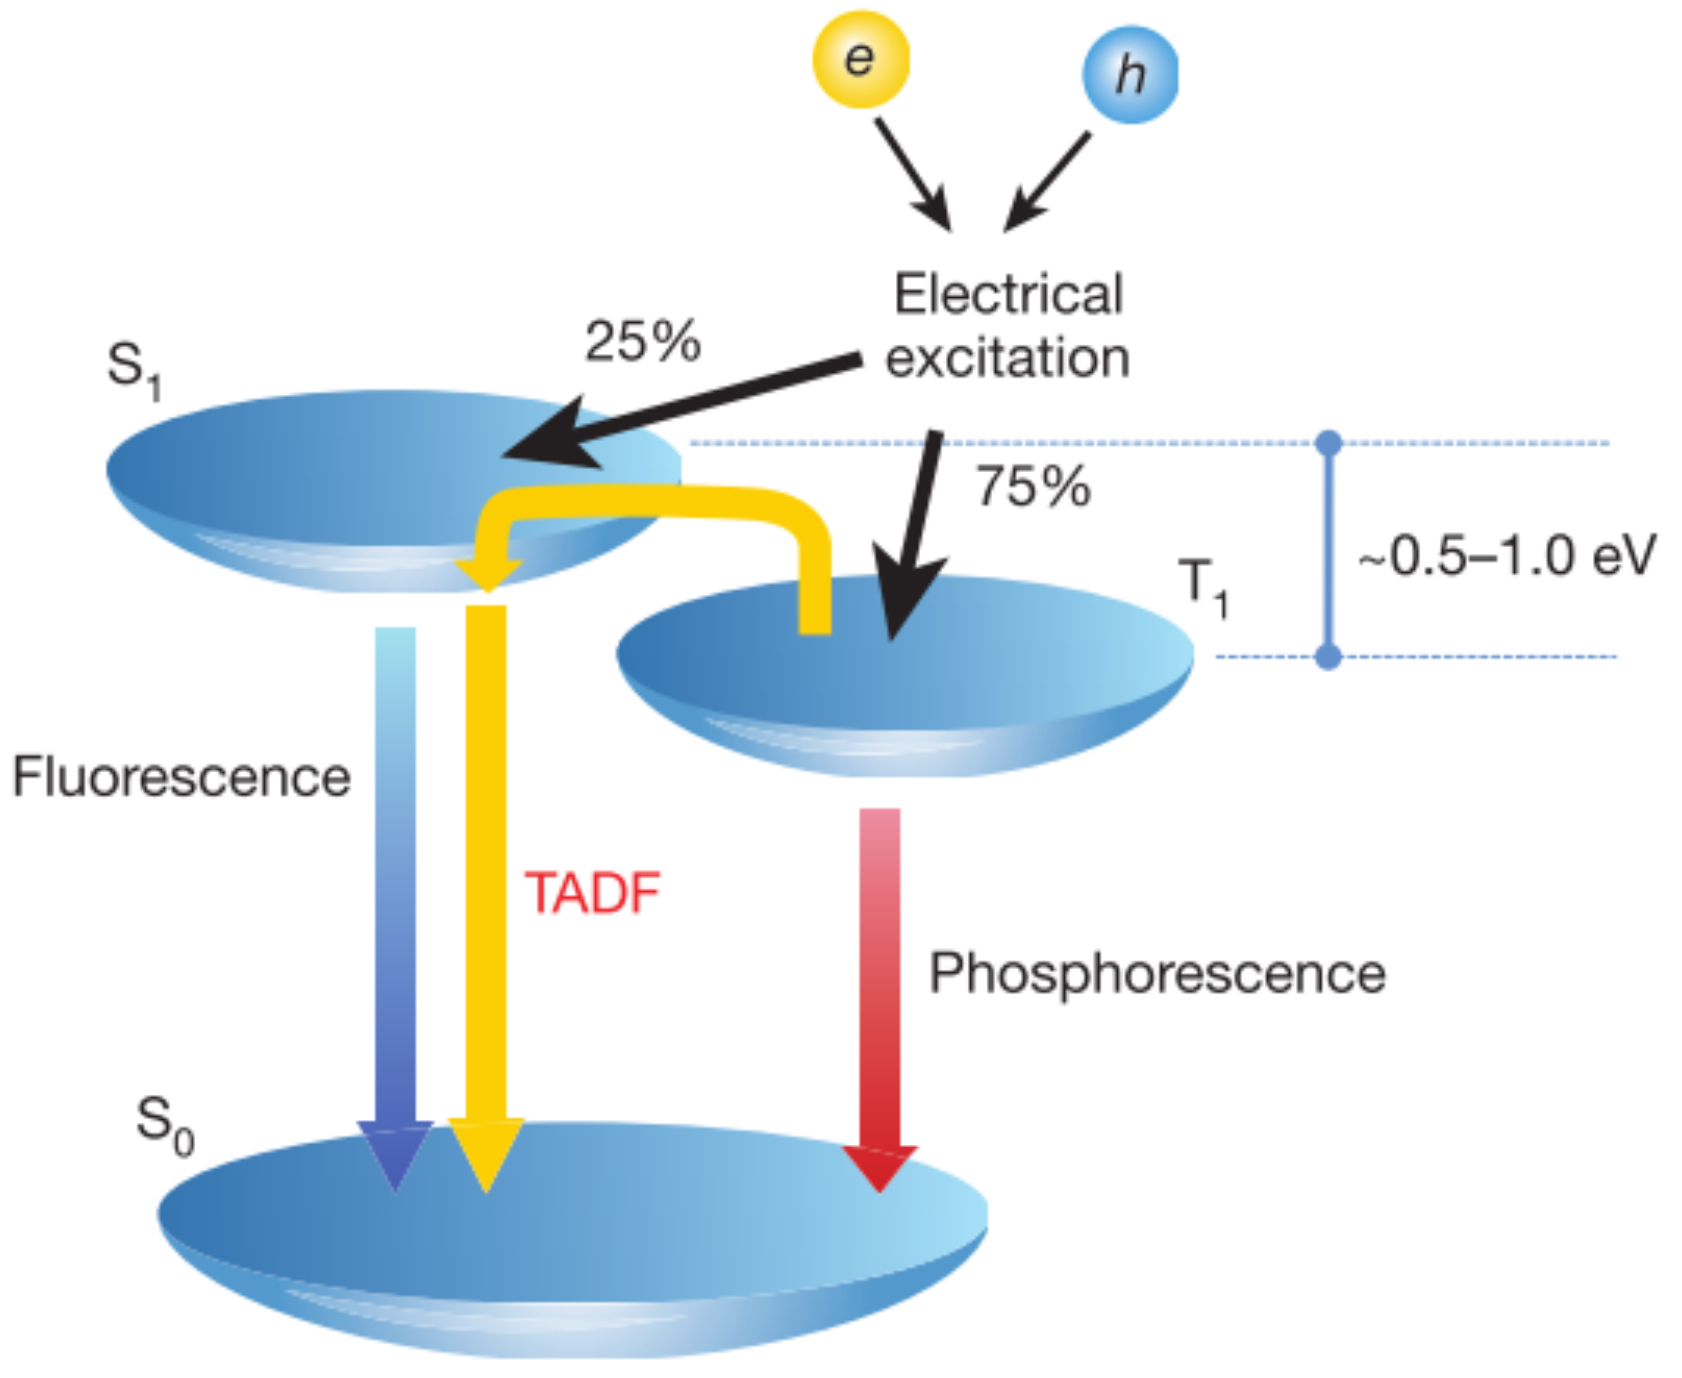
\includegraphics[width=.48\textwidth]{oleds/tadf}
\caption{Reverse intersystem crossing for TADF materials.  Figure taken from \textcite{Uoyama2012}.}
\label{fig:oleds_tadf}
\end{wrapfigure}

While phosphorescent devices have been able to demonstrate high efficiency necessary for commercialization, this has come at a cost.
Namely, in the use of expensive and rare heavy metal atoms, such as Ir(III), Pt(III), and Os(II).\supercite{Adachi2001b}
In order to utilize the triplet excitons, reverse intersystem crossing is utilized.
Chapter \ref{sec:excitons} and Figure \ref{fig:orgSemi_jablonski} discuss intersystem crossing as an energetically favorable process as the triplet is lower energy than the singlet.
However, if molecules are designed where the singlet and triplet energies difference ($\Delta E_{ST}$) is small ($<1eV$), thermal energy can make the reverse intersystem crossing competitive with intersystem crossing ($k_{RISC}\approx k_{ISC}$).
This allows for Thermally Activated Delayed Fluorescence (TADF), shown in Figure \ref{fig:oleds_tadf}.\supercite{Zhang2012b,Zhang2014a,Uoyama2012}
TADF materials are a rapidly developing technology that has shown many benefits for efficiency, and rules are being established for molecular design.\supercite{Menke2016,Inoue2016,Li2013,Wang2015,Liu2015,Kim2015,Jankus2014,Lavie-Cambot2008,Zhang2012b,Endo2009,Yersin2014,Nasu2013,Uoyama2012,Zhang2012c,Hofbeck2015,Linfoot2014,Reineke2014a,Zhang2014a}
These materials are also being investigated for benefits to device lifetime.\supercite{Mehes2014,Cho2014}


\section{Efficiency Roll-Off}\label{sec:oleds_roll_off}
\begin{wrapfigure}{r}{.5\textwidth}
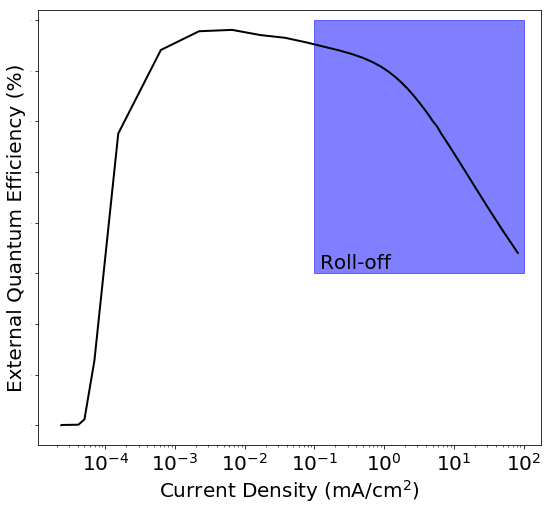
\includegraphics[width=.48\textwidth]{oleds/roll_off}
\caption{Efficiency roll-off as a function of current density}
\label{fig:oleds_rolloff}
\end{wrapfigure}

In operational OLEDs, it is almost universally observed that efficiency reduces at high brightness and current density, an affect known as the efficiency roll-off,demonstrated in Figure \ref{fig:oleds_rolloff}.\supercite{Erickson2014,Song2011,Wehrmeister2015,Son2008,Murawski2013,Giebink2008c,Song2010,Xiang2016,Coehoorn2015,Reineke2009,Mezyk2005,Baldo2000a,Reineke2007,Kohler2009,Hershey2016,Erickson2013a}
This has been extensively studied and largely attributed to the bimolecular quenching processes discussed in Chapter \ref{sec:excitons}, though exciton formation efficiency (\ef) is also known to contribute at a lesser degree.
This is detrimental to commercialization as high brightness is a necessity for display and lighting applications.
The bimolecular quenching at high brightness is also detrimental to device lifetime because quenching processes produce hot excited states that release excess energy into the device, which is thought to be a key factor in molecular degradation.\supercite{Giebink2008a,Coburn2017,Lee2017}
Developement of electrically pumped organic lasers has proved unsuccesful because the exciton densities required to achieve population inversion lead to excessive quenching and the inability to create stimulated emission.\supercite{Baldo2002,Baldo1998a,Holmes2007,Takenobu2008,Samuel2009,Kasemann2011}

Devices are often investigated to try to reduce the roll-off, often through the broadening of the exciton recombination zone.\supercite{Wang2015,Murawski2014,Inoue2016,Soofi2017,Chopra2010,Reineke2007a,Lee2009b,Su2008a,Zang2008}
These devices have not been successful in removing the roll-off, but rather in reducing it.
Section \ref{sec:oled_operation} discussed the characterization of quantum efficiency using a four component efficiency model.  
This model fails to reproduce the roll-off behavior as it does not account for quenching.
Modeling the efficiency roll-off has been the study of numerous works and is the motivation for Chapter \ref{sec:unified}.\supercite{Reineke2007,Erickson2014,Hershey2016,Murawski2013}
These models center around a differntial equations model for exciton dynamics, such as:

\begin{equation}
\frac{dn_{ex}}{dt} = - \frac{n_{ex}}{\tau}-\frac{1}{2}\ktt n_{ex}^2-\ktp n_{pol}n_{ex}+G_{ex}
\label{eqn:oleds_exciton_rate}
\end{equation}

where $n_{ex}$ is the exciton population density, $\tau$ is the exciton lifetime, \ktt is the triplet-triplet annihilation rate, \ktp is the triplet-polaron quenching rate, $n_{pol}$ is the charge density, and $G_{ex}$ is the exciton genertion rate.
Here we can see that the natural lifetime is competitive with the bimolecular quenching rates, and at high exciton and charge density, the second order dependence of the quenching terms allows them to dominate.
This reduces the relative number of excitons that are decaying via the radiative rate, thus decreasing the efficiency.
These models have been successfull in characterizing the rate constants and describing the roll-off behavior.
For further details, see Chapter \ref{sec:unified}.


\section{Recombination Zone Characterization}\label{sec:rz_measurement}
\begin{wrapfigure}{r}{.5\textwidth}
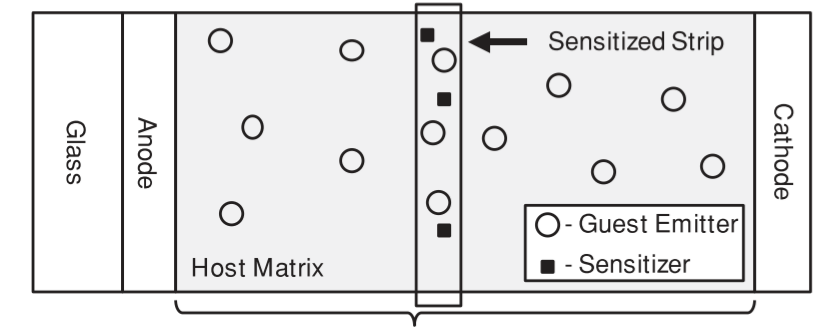
\includegraphics[width=.48\textwidth]{oleds/rz_arch}
\caption{Recombination zone measurement architecture.  The curly brace indicates the device stack.  Figure taken from \textcite{Erickson2013a}}
\label{fig:oleds_rz_arch}
\end{wrapfigure}
Both degradation and bimolecular quenching can be highly dependent on the exciton density and location, known as the exciton recombination zone (RZ).\supercite{Giebink2006,Giebink2008a,Giebink2008c,Giebink2009a,Reineke2007,Hershey2016,Hershey2017,Bangsund2018}
Therefore, it is important to be able to characterize the spatial profile of excitons.
This has been done by a variety of researchers using thin doping layers of a sensitizer molecule.\supercite{Reineke2007a,Coburn2016a,Coburn2017,Erickson2013a,Hershey2017,Bangsund2018}

In these experiments, the dopant is used to efficienctly siphon excitons off of the emitter molecule and onto the sensitizer.
In order to do this, F\"{o}rster transfer to the sensitizer must be efficient, requiring significant overlap of the emitter emission and the sensitizer absorption.
\textcite{Erickson2013a} looked at the spatial extent of F\"{o}rster transfer and found that transfer was efficient within a $<4$ nm radius.
To characterize the recombination zone, sensitized layers are used and the effect of the local perturbation of the exciton density can be measured.
Translating the sensitized strip across the device as shown in Figure \ref{fig:oleds_rz_arch} allows for comparison of the relative effects and thus determination of the relative magnitude of the recombination zone.
The F\"{o}rster radius gives the maximum spatial resolution that can be obtained using this strip translation.

A quenching (non-radiative) or emissive (radiative) sensitizer can be used for these experiments.
With a quenching sensitizer, if the recombination zone overlaps with the sensitizer position, emission is lost and the efficiency is reduced.
The reduction in EL intensity can be quantified by the EL ratio of the sensitized intensity compared to the unsensitized intensity, $\beta$.
$\beta$ is directly proportional to the unquenched excitons, therefore $1-\beta$ gives the ratio of quenched excitons.

For emissive sensitizers, given the requirement of emission-absorption overlap, red sensitizers are used.
For simplicity, the sensitizer should show spectral separation of the emission from the emitter.
The intensity of the sensitizer emission is a direct measure of the local exciton density.
However, since the out-coupling is so strongly dependent on emitter position in the EML, it is essential to correct the intensity using a calculation of \oc, discussed in Chapter \ref{sec:out_coupling}.
One may note that the quenching sensitizer method should also require out-coupling correction, but since the emission is not spatially isolated, calculation of the spatially averaged out-coupling effiency would require prior knowledge of the recombination zone shape and therefore cannot be done.
Emissive sensitizers often rely on the use of Pt(II) complexes, such as PtOEP or PtTPTBP.\supercite{Coburn2016a,Hershey2017}
Compared with Ir(III) complexes, Pt(II) shows a much longer exciton lifetime, and is therefore far more sucesptible to bimolecular quenching.\supercite{Mezyk2005}
If the sensitizer is in a regime of bimolecular quenching during the measurement, a compressed version of the recombination zone will be measured.
This can be difficult to avoid at high current densities that may be of interest for measurement.

\begin{wrapfigure}{r}{.5\textwidth}
\includegraphics[width=.48\textwidth]{oleds/rz_comparison}
\caption{Recombination zone comparison for an emissive sensitizer analyzed using the quenched ratio and the emitted ratio as a function of current density.}
\label{fig:oleds_rz_comparison}
\end{wrapfigure}

An advantage of the emissive sensitizer is that the data generated can be analyzed either using the quenched ratio or using the emitted intensity.
This can be helpful for quantifying error in the method, and is demonstrated in Figure \ref{fig:oleds_rz_comparison}.
Here, we see the spatial dependence of the recombination zone for an architecture peaked at the ETL interface.
Notice that the emissive sensitizer, PtTPTBP shows a less exaggerated RZ for all current densities.  
This is likely due to bimolecular quenching on the sensitizer, which is stronger at the higher exciton densities present at the ETL interface.

When constructing these sensitizer layers, there are two popular methods.  
First, the EML can be reproduced exactly with the addition of a light doping of the sensitizer.  
This creates a strip that exactly replicates EML, but increases the difficulty of the growth, requiring one more material in a codeposition.
An alternative is to use an extremely thin deposition of the sensitizer molecule in isolation, known as delta doping.
A deposition of 1 \r{A} is used, which since the molecular radius of the deposited material is larger than that, in reality, a discontinuous layer is produced.
When the EML is continued on top of this discontinous layer, this is equivalent to an extremely narrow strip of a mixed layer.
This is advantagous because it make the deposition much easier and creates a very narrow strip.
However, it can be difficult to control the doping percentage as it is difficult to accurately measure films this thin.
No quantification of error on these types of doping have been reported.

In order to accurately compare the recombination zone intensity, it is essential to ensure that no differences in the transport and injection properties occur with the introduction of the sensitizer.
Since the sensitizer molecules will likely result in a trap state, it is essential to keep doping concentrations low, on the order o 1\%.
Evidence of minimal interference on the electrical properties by the sensitizer is provided by the current-voltage behavior.
If the current-voltage characteristic is within error between all of the sensitizer devices, it is often assumed that the device is representative of the control.\supercite{Erickson2013a}

\section{Single Carrier Devices}

\section{Operational Lifetime}
In typical lifetime characterization, devices are degraded while held at constant current density, recording the resulting luminance loss and voltage gain as a function of time.  
The lifetime is then reported as the time to reach some arbitrary fraction of the initial luminance.

\begin{equation}
\frac{L(t)}{L_0}=\exp (t/\tau)^\beta
\label{eqn:stretched_exponential}
\end{equation}



\subsection{Degradation Mechanisms}\label{sec:degradation_mechanisms}

As degradation studies are an ongoing an extensive aread of research, this section does not represent an all inclusive picture of degradation mechanisms.  However, it does seek to outline the dominant mechanisms observed in typical devices.
In the most simple case, the degradation of an OLED can be viewed wholistically as a stretched exponential curve with minimal physics.\supercite{Scholz2015,Fry2005a}
This approach is able to reproduce the decay behavior relatively well and the scaling with luminance, but only describes the decay by attributing behavior to emissive centers.

\subsubsection{Dark Spots and Delamination}



\subsubsection{Exciton and Polaron}
\subsubsection{Interfaces}
\subsubsection{Oxygen}


\subsection{Luminance Scaling}\label{sec:luminance_scaling}
For commercially relevant devices, where the time to reach 50\% of the initial luminance, $t_{50}$ can be tens of thousands of hours, it is impractical to test devices under their intended operating conditions.
Instead, lifetime testing can be done at an increased luminance from the true operating condition.\supercite{Scholz2015}
This can dramatically reduce the testing time of devices.
The lifetime at other luminances can then be found using the scaling relation

\begin{equation}
L_0^n t_x=C
\label{eqn:luminance_scaling}
\end{equation}

where $L_0$ is the initial luminance, $n$ is a scaling factor characteristic to the device, and $C$ is a constant.
To utilize this relation, several lifetimes are obtained at luminances above the operating condition in order to experimentally obtain a value for $n$.
Subsiquently, the lifetime of interest can then be extrapolated.

While widely used and observed, caution should be observed in the application of this relation.  
A variety of degradation mechanisms have been attributed to OLED behavior, as discussed in Section \ref{sec:degradation_mechanisms}.
All of these mechanisms are subject to different temporal dependences and have a variety of degrees of understanding to their fuctional dependence on time and luminance.
At different luminances, different mechanisms may be dominant.
For example, single excitonic processes may be dominant at low luminance, but may be overtaken by a bimoleculat process at high luminance.
The fact that OLEDs are frequently subject to several degrdation mechanisms throughout the decay only further complicates the issue.
The very idea of scaling law for all devices and at all current densities is unsound, and should be treated as a loose prediction.
Over and underestimates of lifetimes using this relation are observed when trying to predict actual lifetimes.\supercite{Meerheim2006,Fry2005}


\subsection{Analysis Techniques}\label{sec:degradation_analysis}




\ifcsdef{mainfile}{}{\printbibliography}
\end{document}
